% Template file for an a0 portrait poster.
% Written by Graeme, 2001-03 based on his SOC poster.
%
% See discussion and documentation at
% <http://www.astro.gla.ac.uk/users/norman/docs/posters/> 
%
%%%%%%%%%%%%%%%%%%%%%%%%%%%%%%%%%%%%%%%%
% Modified by Jozef Dobo\v{s} (c) 2011 % 
%%%%%%%%%%%%%%%%%%%%%%%%%%%%%%%%%%%%%%%%

\documentclass[a0,portrait]{a0poster}
% You might find the 'draft' option to a0 poster useful if you have
% lots of graphics, because they can take some time to process and
% display. (\documentclass[a0,draft]{a0poster})

\pagestyle{empty}
\setcounter{secnumdepth}{0}
\usepackage[absolute,
					%showboxes
					]{textpos}
\usepackage{txfonts}
\usepackage{wrapfig,times}
\usepackage[scaled]{helvet}
\usepackage{graphicx}
\usepackage{forloop}
\usepackage[margin=0cm]{geometry}
\usepackage{wasysym}
\usepackage{enumitem}
\usepackage{tipa}
\usepackage{tikz}
\usetikzlibrary{backgrounds}


%%%%%%%%%%
% Colors %
%%%%%%%%%%
\usepackage{color}
\definecolor{TitleColor}{rgb}{1,1,1} % white
\definecolor{BannerOneColor}{rgb}{0,0,0} % pitch black
\definecolor{BannerTwoColor}{rgb}{0.93,0.08,0.31} % pinky red
\definecolor{BannerThreeColor}{rgb}{0,0.27,0.48} % dark blue
\definecolor{BannerFourColor}{rgb}{0.33,0.19,0.098} % brown
\definecolor{BannerSixColor}{rgb}{0,0.27,0.42} % dark blue
\definecolor{BannerSevenColor}{rgb}{0.62,0.77,0.86} % sky blue
\definecolor{BannerEightColor}{rgb}{0.35,0.33,0.01} % military green
\definecolor{BannerNineColor}{rgb}{0.85,0.86,0.34} % lime green
\definecolor{BannerTenColor}{rgb}{0,0.66,0.80} % strong blue
\definecolor{BannerElevenColor}{rgb}{0.46,0,0.20} % maroon
\definecolor{BannerTwelveColor}{rgb}{0.37,0.32,0.44} % dark washed violet
\definecolor{BannerThirteenColor}{rgb}{0.79,0.84,0.65} % light washed green
\definecolor{BannerFourteenColor}{rgb}{0.57,0.64,0.27} % dark washed green
\definecolor{BannerFifteenColor}{rgb}{0.92,0.91,0.88} % unusable washed 
\definecolor{BannerSixteenColor}{rgb}{0.94,0.36,0.14} % strong orange
\definecolor{BannerSeventeenColor}{rgb}{0.97,0.61,0.19} % orange
\definecolor{BannerEighteenColor}{rgb}{0.99,0.76,0.11} % mustard yellow
\definecolor{BannerNineteenColor}{rgb}{0.79,0.76,0.73} % light gray-ish
\definecolor{BannerTwentyColor}{rgb}{0.63,0.58,0.54} % dark gray-ish

\def\bannercolor{BannerSixColor}

%%%%%%%%%%%%%%%%%%%%%%%%%%%%%%%%%%%%%%%%%%%%%%%%%%%%%%
% Only change here to affect all headings            %
\newcommand{\headingcolor}{\color{BannerSixColor}} 
\newcommand{\titlecolor}{\color{TitleColor}}
%\newcommand{\banner}{\includegraphics[width=\linewidth]{banners/darkblue.pdf}}
\newcommand{\banner}{\LARGE \tikz{\path[draw=\bannercolor,fill=\bannercolor] (0,0) rectangle (\linewidth,2.25em);}}
\def\Highlight#1{{\sffamily \headingcolor #1}}
%%%%%%%%%%%%%%%%%%%%%%%%%%%%%%%%%%%%%%%%%%%%%%%%%%%%%%

% see documentation for a0poster class for the size options here
\let\Textsize\Large
\def\Head#1{\noindent\hbox to \hsize{\hfil{\LARGE \headingcolor #1}}\bigskip}
\def\LHead#1{\noindent{\sffamily \LARGE \headingcolor #1}\smallskip}
\def\Authors#1{\noindent{\sffamily \LARGE #1}\smallskip}
\def\Subhead#1{\noindent{\large \headingcolor #1}}
\def\Title#1{\noindent{\sffamily \VeryHuge \titlecolor #1}}

\setlist[itemize,1]{topsep=0pt, label={{\headingcolor $\bullet$}}}
\setlist[itemize,2]{topsep=0pt, label={{\headingcolor $\triangleright$}}}
%\setitemize{topsep=0pt}

% Set up the grid
%
% Note that [0cm,0cm] is the margin round the edge of the page --
% it is _not_ the grid size. That is always defined as 
% PAGE_WIDTH/HGRID and PAGE_HEIGHT/VGRID. In this case we use
% 25 x 25. This gives us three wide columns for text (7 grid
% spacings) and four narrow columns (1 each) at each side of these 
% text columns
%
% Note however that texblocks can be positioned fractionally as well,
% so really any convenient grid size can be used.
%

% [margin, margin]{rows}{cols}
\TPGrid[0cm,0cm]{17}{25}  % 1 - 7 - 1 - 7 - 1 Columns


% Mess with these as you like
\parindent=0pt
%\parindent=1cm
\parskip=0.5\baselineskip
\linespread{1.2}

% abbreviations
\newcommand{\ddd}{\,\mathrm{d}}

\begin{document}

% Understanding textblocks is the key to being able to do a poster in
% LaTeX. In
%
%    \begin{textblock}{width}(x,y)
%    ...
%    \end{textblock}
%
% the first argument gives the block width in units of the grid
% cells specified above in \TPGrid; the second gives the (x,y)
% position on the grid, with the y axis pointing down.

%%%%%%%%%%%%%%
% Top Banner %
%%%%%%%%%%%%%%


%\begin{tikzpicture}[remember picture, overlay]
%\begin{pgfonlayer}{background}
%  \path[draw=BannerTwelveColor,fill=BannerTwelveColor] (0,0) rectangle (\paperwidth,9cm);
%\end{pgfonlayer}
%\end{tikzpicture}

 %if you change this part, you can get matching color for headings
 %in Colors section above
\begin{textblock}{17}(0,0) {
%\includegraphics[width=\paperwidth]{banners/darkblue.pdf}
%\includegraphics[width=\paperwidth]{banners/purple.pdf}
\VeryHuge
\tikz{\path[draw=\bannercolor,fill=\bannercolor] (0,0) rectangle (\paperwidth,2.75em);}
} \end{textblock}




%%%%%%%%%
% Title %
%%%%%%%%%
%TODO MAKE TITLE BANNER BIGGER/LESS CRAMPED
\begin{textblock}{10}(1,0.25)
{\color{TitleColor}
\Title{A CAPT tool for training and research on lexical stress errors in German}\\

%\Authors{Anjana Vakil}, {\sffamily \Large Computational Linguistics}\\
%\textbf{\large \texttt{anjanav@coli.uni-saarland.de}}
}
\end{textblock}

\begin{textblock}{4}(12,0)    
\begin{flushright}
%\resizebox{1.5\TPHorizModule}{!}{

\includegraphics[width=1.3\TPHorizModule]{../../../img/new-owl-white.png}
%
\includegraphics{images/saarland_university_white.png}
%
\includegraphics{images/uds-logo-text-white.png}
\end{flushright}
\end{textblock}

\begin{textblock}{4}(10.5,0.2){
\color{TitleColor}
\begin{flushright}
\Authors{Anjana Vakil}\\
{\sffamily \Large Computational Linguistics}\\%, Saarland University}\\
{\sffamily \Large Saarland University}\\
\textbf{\large \texttt{anjanav@coli.uni-saarland.de}}
\end{flushright}
}
\end{textblock}

%\begin{textblock}{5}(1,2){
%\headingcolor
%\Authors{Anjana Vakil}\\
%{\sffamily \Large Computational Linguistics, Saarland University}\\%, U. Saarland}\\
%\textbf{\large \texttt{anjanav@coli.uni-saarland.de}}
%}
%\end{textblock}




% An example text block, to get you started!
\begin{textblock}{7}(1, 2.25) {
\banner
} \end{textblock}
\begin{textblock}{6.75}(1.25,2.5){
  \LHead{\titlecolor Introduction}}
 \end{textblock}
 \begin{textblock}{7}(1, 3.25)
  \Textsize
Computer-Assisted Pronunciation Training (CAPT) can:
\begin{itemize}
\item{automatically analyze and diagnose pronunciation errors}
\item{offer individualized feedback on errors and how to correct them}
\item{complement traditional classroom-based language study\\(which typically neglects pronunciation teaching)}
\item{encourage independent study}
\end{itemize}

This poster describes upcoming work towards the development of a CAPT system targeting native (L1) French speakers learning German as a foreign language (L2).

\Highlight{Context:} M.Sc. thesis, related to ongoing Franco-German project\\ \textit{Individualized Feedback for Computer-Assisted Spoken Language\\ Learning} (IFCASL) [3].
% at University of Saarland (Saarbr{\"u}cken, Germany) and LORIA (Nancy, France).
 
\Highlight{Aim:} Engineer a {prototype German CAPT system} offering L1 French speakers feedback on one type of pronunciation error.
 
%\Highlight{Intended contributions:} 
%\begin{itemize}
%\item{Survey and build upon existing research on automatic diagnosis and correction of errors in L2 German speech}
%\item{Engineer a {prototype German CAPT system} offering L1 French speakers feedback on one type of pronunciation error}
%\end{itemize}

%\end{textblock}
%
%
%\begin{textblock}{7}(1, 7.25) {
%\banner
%} \end{textblock}
%\begin{textblock}{6.75}(1.25,7.5){
%  \LHead{\titlecolor Main research questions}}
% \end{textblock}
% \begin{textblock}{7}(1, 8)
%  \large
  
The work has {3 main research questions}, outlined below.
%\begin{enumerate}
%\item{Which error(s) should a German CAPT system address?}
%\item{How can this type of error best be automatically diagnosed?}
%\item{How can helpful feedback on this error be automatically given to learners?}
%\end{enumerate}
\end{textblock}

\begin{textblock}{7}(1, 10.25) {
\banner
} \end{textblock}
\begin{textblock}{6.75}(1.25,10.5){
  \LHead{\titlecolor 1. Which error should the system address?}}
 \end{textblock}
 \begin{textblock}{7}(1, 11.25)
\Textsize
\Highlight{Goal:} Determine which type of L2 German pronunciation errors 
%(including segmental errors and prosodic deviations) 
is best addressed by a CAPT system.

\Highlight{Criteria for error selection:} An error is a good CAPT target if it...
\begin{itemize}
%\renewcommand{\labelitemi}{$\RHD$}
\item{is frequently produced by L2 speakers (with French as L1)}
\item{affects (perceived) intelligibility of learner's speech}
\item{can be reliably detected/diagnosed automatically}
\end{itemize}

\begin{center}
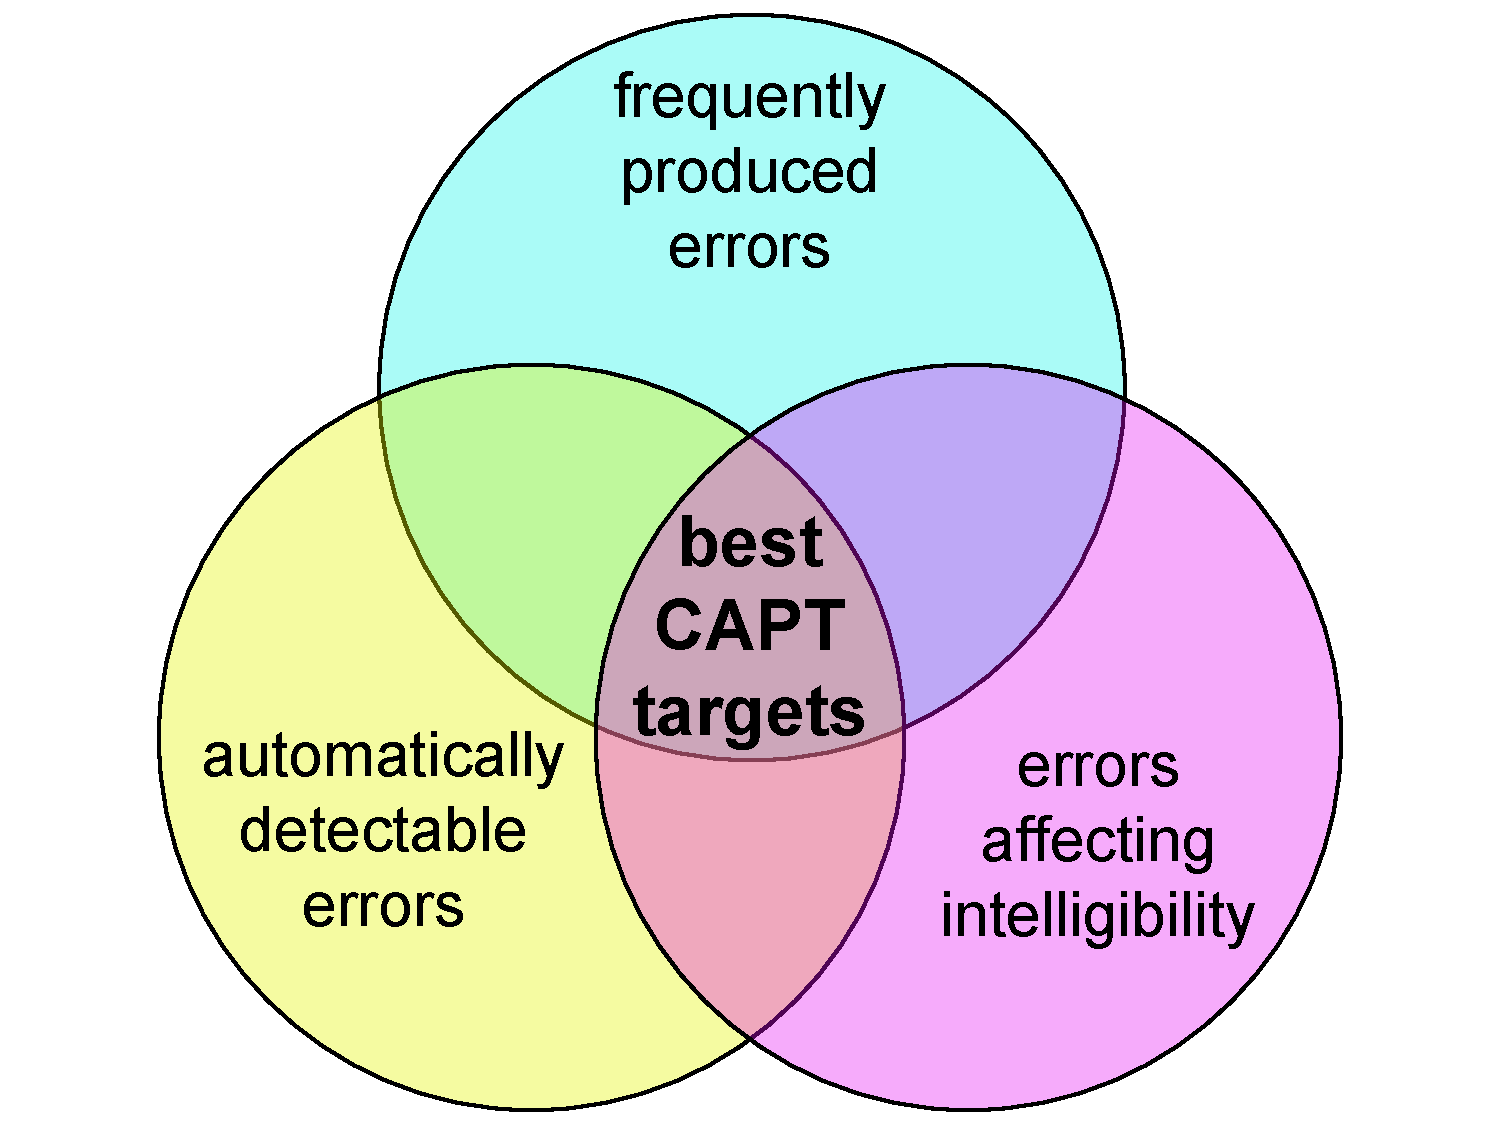
\includegraphics{../../../img/error-venn.pdf}
\end{center}

\Highlight{Proposed methods for selecting target error type(s):}
\begin{itemize}
\item{Analysis of subset of IFCASL corpus (spoken L1/L2 German) [3]}
\item{Survey of past research on L2 intelligibility (e.g. [2])}
\item{Survey of past research on CAPT/L2 speech processing (e.g. [1])}
\end{itemize}

\Highlight{Hypothesized errors fitting the criteria:}
\begin{itemize}
\item{Lexical accent errors [1,2], such as:
		\begin{itemize}
		\item{Stress on wrong syllable (e.g. [\textipa{"apKIl}] vs. [\textipa{a"pKIl}])}
		\item{No distinction between stressed/unstressed syllables}
		%\item{Lack of reduction of unstressed syllables}
		\end{itemize}}
\item{Vowel quality and/or quantity errors, e.g. [\textipa{i}] for /\textipa{I}/ or /\textipa{i:}/}
\end{itemize}

\end{textblock}


\begin{textblock}{7}(9, 2.25) {
\banner
} \end{textblock}
\begin{textblock}{6.75}(9.25,2.5){
  \LHead{\titlecolor 2. How can the error be automatically diagnosed?}}
 \end{textblock}
 \begin{textblock}{7}(9, 3.25)
  \Textsize
  
\Highlight{Goal:} Given target error, determine best technique for automatically detecting this error in L2 speech.

\Highlight{Criteria for technique selection:} Automatic diagnosis must be...
\begin{itemize}
%\renewcommand{\labelitemi}{$\RHD$}
\item{reliable (i.e. of reasonably high accuracy)}
\item{fast on modern consumer-grade hardware\\(to generate diagnosis and feedback within seconds)}
\end{itemize} 

\Highlight{Proposed methods for determining best technique:}
\begin{itemize}
\item{Survey of research into automatic processing of this phenomenon}
\item{Comparison of existing techniques}
\item{Experimentation with new techniques (if needed)}
\end{itemize}

  
\end{textblock}


\begin{textblock}{7}(9, 8.5) {
\banner
} \end{textblock}
\begin{textblock}{6.75}(9.25,8.75){
  \LHead{\titlecolor 3. What feedback can/should learners receive?}}
 \end{textblock}
 \begin{textblock}{7}(9, 9.5)
  \Textsize
  
\Highlight{Goal:} Given target error and processing technique(s), develop one or more methods to model mastery and deliver feedback. Ideally:
\begin{itemize}
\item{develop multiple feedback options}
\item{determine best feedback type dynamically based on learner-specific factors (e.g. skill level)}
\end{itemize}

\vspace{1em}

\begin{center}
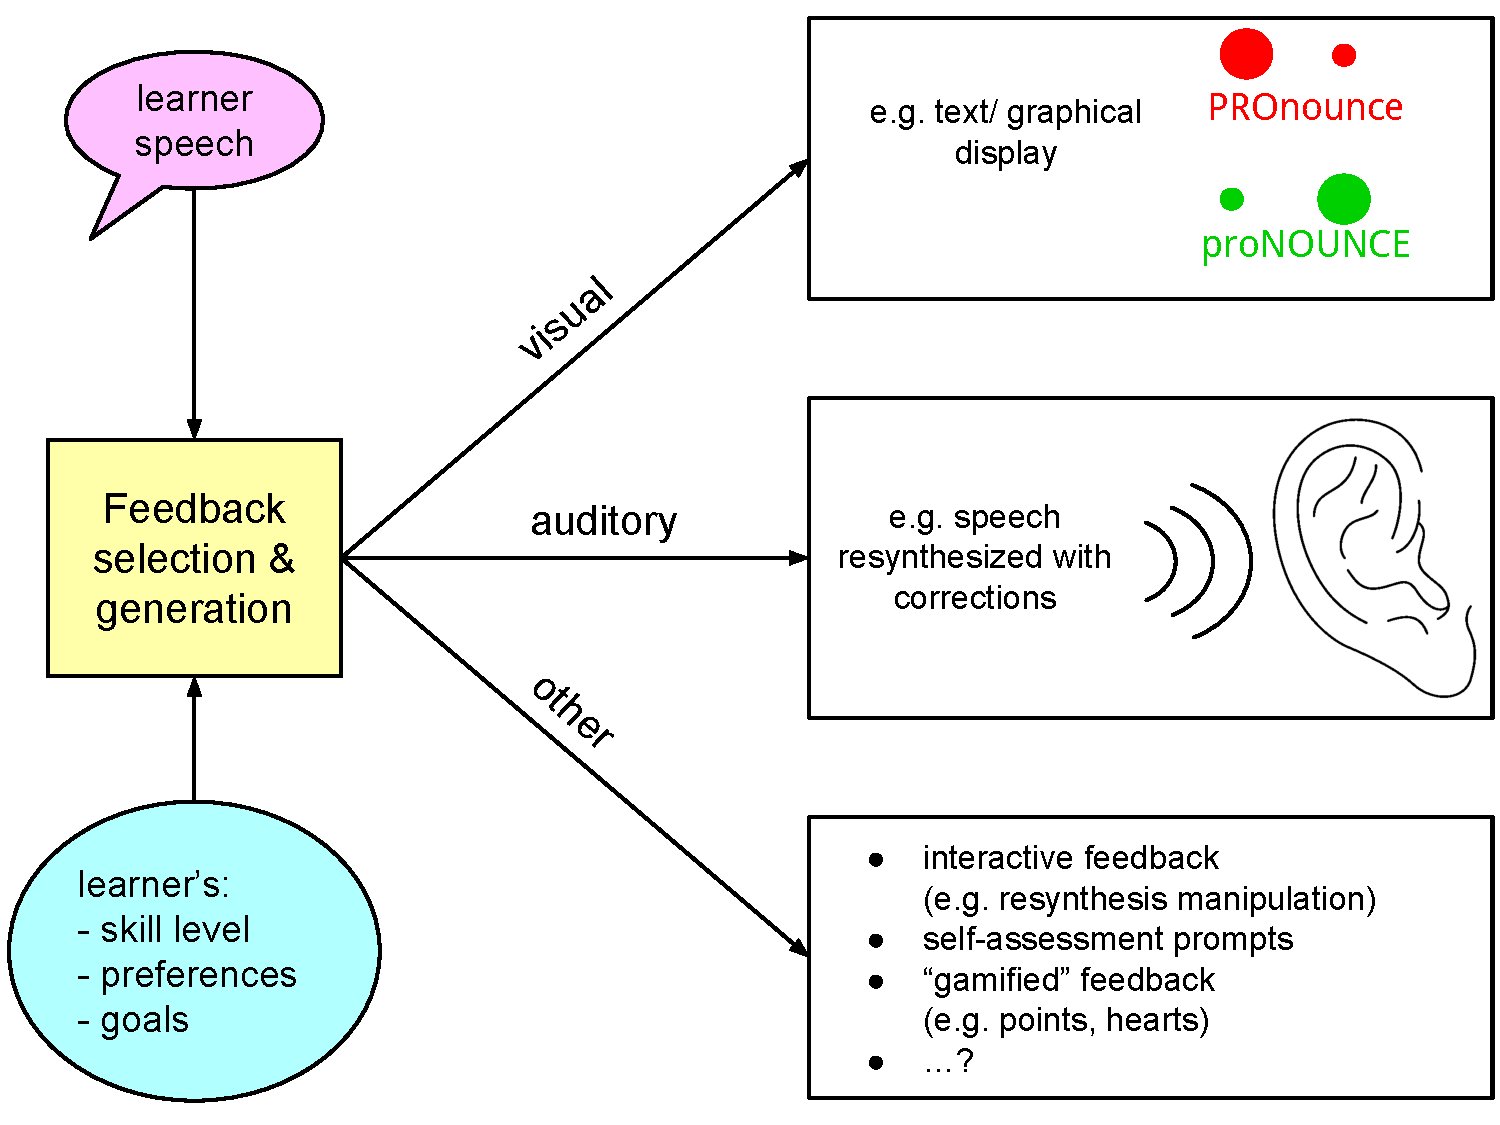
\includegraphics{../../../img/feedback.pdf}
\end{center}
%\Highlight{Proposed methods for developing feedback:}
%\begin{itemize}
%\item{Survey of past studies on CAPT feedback (e.g. [1])}
%\item{Experimentation with new feedback strategies}
%\end{itemize}

 
\end{textblock}

%\begin{textblock}{7}(9,2)
%\newcounter{int}
%\begin{enumerate}
%\forloop{int}{1}{\value{int} < 21}{
%\item \includegraphics[width=0.98\linewidth]{banners/banner\arabic{int}.pdf}
%}
%\end{enumerate}
%\end{textblock}


% Another text block in the bottom right.
\begin{textblock}{7}(9,17){
\banner
} \end{textblock}
\begin{textblock}{6.75}(9.25,17.25){
  \LHead{\titlecolor Conclusion}
   } \end{textblock}
 \begin{textblock}{7}(9, 18)
  \Textsize
  
\Highlight{Outcome:} Prototype CAPT system for the selected error type, implementing the chosen analysis and feedback method(s).

If successful, the prototype will be integrated into the more comprehensive CAPT system developed in the IFCASL project.

\Highlight{Intended contribution:} Survey and build upon existing research on automatic diagnosis and correction of errors in L2 German speech.
  
\Highlight{Possible extension:} Evaluate the effect of given feedback type(s) on:
\begin{itemize}%[topsep=0pt,parsep=0pt,partopsep=0pt]
\item{Production/mastery of the error}
\item{Satisfaction with the prototype CAPT system}
\item{Motivation to use the system}
\end{itemize} 

\end{textblock}


\begin{textblock}{15}(1,23)
{\Large
\tikz{\path[draw=\bannercolor,fill=\bannercolor] (0,0) rectangle (\linewidth,2em);}}
\end{textblock}
\begin{textblock}{14.75}(1.15,23.15)
\LHead{\Large \titlecolor References}
\end{textblock}
\begin{textblock}{15}(1,23.55)
\begin{enumerate}[label={[\arabic*]}, leftmargin=34pt, topsep=0pt]
\item{Bonneau, A. and Colotte, V. 2011. “Automatic Feedback for L2 Prosody Learning”. In \textit{Speech and Language Technologies}. Ivo Ipsic, ed. InTech.}

\item{Hirschfeld, U. 1994. \textit{Untersuchungen zur phonetischen Verst{\"a}ndlichkeit Deutschlernender.} Forum Phoneticum, 57.}

\item{Trouvain, J., et al. 2013. ``Designing a bilingual speech corpus for French and German language learners''. \textit{Proc. Corpus et Outils en Linguistique, Langues et Parole}, Strasbourg, pp. 32-34.}
\end{enumerate}

\end{textblock}

%\begin{textblock}{15}(1,23.25)
%\LHead{\Large \headingcolor References}
%\begin{enumerate}[label={[\arabic*]}, leftmargin=34pt, topsep=0pt]
%\item{Bonneau, A. and V. Colotte. 2011. “Automatic Feedback for L2 Prosody Learning”. In \textit{Speech and Language Technologies}. Ivo Ipsic, ed. InTech.}
%
%\item{Hirschfeld, U. 1994. \textit{Untersuchungen zur phonetischen Verst{\"a}ndlichkeit Deutschlernender.} Forum Phoneticum, 57.}
%
%\item{Trouvain, J., et al. 2013. ``Designing a bilingual speech corpus for French and German language learners''. \textit{Proc. Corpus et Outils en Linguistique, Langues et Parole}, Strasbourg, pp. 32-34.}
%\end{enumerate}
%
%\end{textblock}


% If you want to add a figure do something like this:

%\begin{textblock}{3}(1,15)
%  \begin{center}
%  \resizebox{3\TPHorizModule}{!}{\includegraphics{images/group-logo.pdf}}
%\\{\bfseries Figure 5:} caption
%  \end{center}
%\end{textblock}



% Place the group logo at the bottom left - visually this balances
% well with the University logo at the top right. 
%\begin{textblock}{4}(1,23)    
%%\resizebox{1.5\TPHorizModule}{!}{
%
\includegraphics{images/uds-logo-text.png}
%%}
%\end{textblock}



\end{document}

